\documentclass{beamer}
\usetheme{TU}


\usepackage[utf8]{inputenc}
\usepackage{ngerman}
\usepackage{german}
\usepackage{amsmath,amsfonts,amssymb}

\begin{document}

\begin{frame}
\frametitle{Free vs. OS vs. Kostenlos}
\begin{figure}
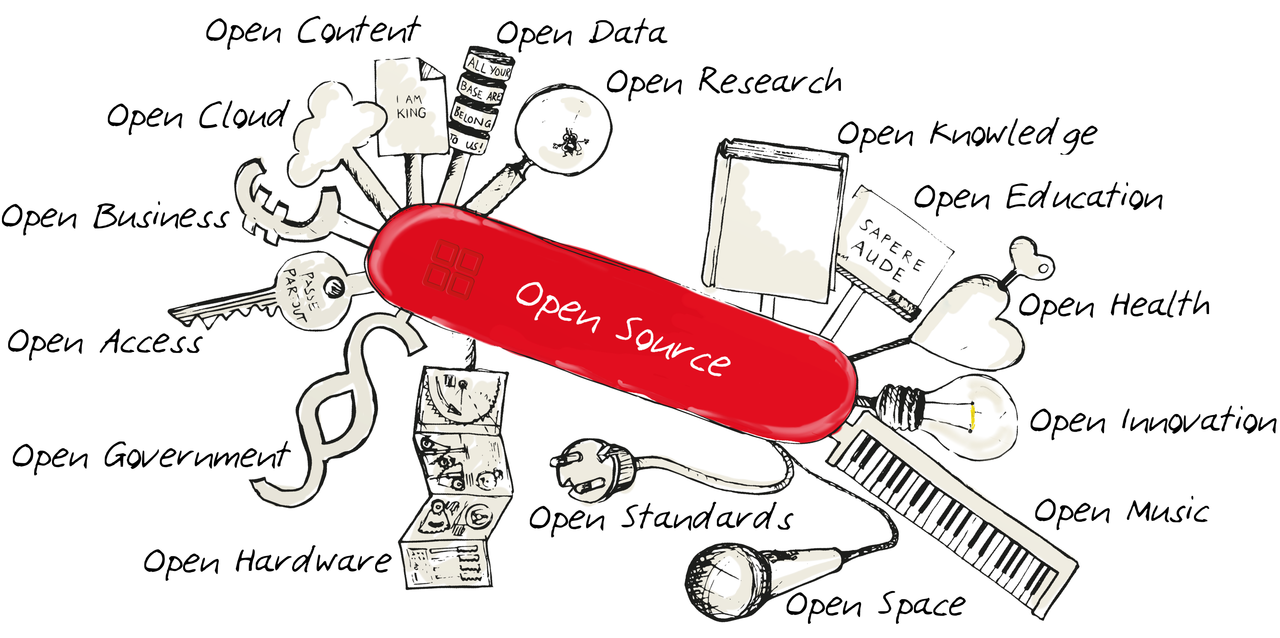
\includegraphics[scale=0.5]{resources/open_swiss_knife.png}
\end{figure}
%Open-Source beschränkt sich nicht nur auf Software
\begin{itemize}
	\item Open-Source == Freies Wissen
	\item Open-Source Software == Software mit frei zugänglichem Quellcode
	\item Free Software:
	\begin{itemize}
		\item 1. Freiheit der Kontrolle über Software
		%totale Kontrolle über alle Aspekte der Software: Analyse und Änderung. Quellcode muss nicht erhalten werden
		\item 2. soziale Freiheit der Kolaboration
		%Verbreitung des Quellcodes. Auch kommerzielle Tätigkeiten dürfen angeboten werden
	\end{itemize}
	\item kostenlose Software (Freeware) == Programmierer verzichtet auf Nutzungsvergütung, nicht auf Urheberrecht
	%Freeware Nutzung wird eingeräumt, Änderung allerdings nicht
\end{itemize}

%\footnote{https://de.wikipedia.org/w/index.php?search=kostenlose+Software&title=Spezial$%$3ASuche&fulltext=Volltext}
\end{frame}

\begin{frame}
\frametitle{Warum ist Open-Source cool?}
\begin{figure}

\includegraphics[scale=0.4]{resources/att.jpg}
\end{figure}
\begin{itemize}
	\item Fehlerbehebung durch Community
	%Bug Hunting
	\item Schwachstellen und potentielle Angriffsstellen werden erkannt
	%Zero-Date exploits, Backdoors
	\item Kontrolle bzgl. unerwünschter Nebenfunktionen
	%Funktionen zur Überwachung oder zur Erstellung von Hintertüren
\end{itemize}
%\footnote{https://www.bing.com/images/search?q=open+source+meme&view=detailv2&&id=3CEEA01A1F60BB879267791D1040EEB7081F26B2&selectedIndex=101&ccid=0j9v2qqY&simid=607986818429160812&thid=OIP.ee0ac8a908656d52412286fa1abe398f&ajaxhis+t=0}
\end{frame}

\begin{frame}
\frametitle{Was ist Linux?}
\begin{figure}

\includegraphics[scale=0.17]{resources/linux.jpg}
\end{figure}
\begin{itemize}
	\item Free, Open-Source Mehrbenutzer-Betriebssysteme
	\item basiert auf dem Linux-Kernel
	%von Linus Torvalds für x86 architecture entwickelt
	%Kernel ist Schnittstelle zwischen Software und Hardware
	%Geschrieben in C
	\item Projekt wird Unterstützt von Unternehmen, Non-Profit-Organisationen und vielen Freiwilligen
	\item Linux-Distro fasst Kernel und unetschiedliche Software zusammen
\end{itemize}
%\footnote{https://ixquick-proxy.com/do/spg/show_picture.pl?l=english&cat=pics&c=pf&q=linux+meme&h=600&w=585&th=227&tw=222&fn=257cc60bfa2c253fc4156db7b9178e8bf510e1812aa9948707c305fd551157bf.jpg&fs=79746%20k&el=googleapi_pics_1&tu=https:$%$2F%2Fs14-eu5.ixquick.com%2Fcgi-bin%2Fserveimage%3Furl%3Dhttp$%$253A%252F%252Ft0.gstatic.com%252Fimages%253Fq%253Dtbn$%$253AANd9GcSj2D3HlI3wpnlNM5DFbH5GaXxcVMvhe3FEIkE8ChCZqZRcOjvJ1g$%$26sp%3De2c7d563e6ebd1ab1aa4e2d46f561fa5&rl=NONE&u=http:%2F$%$2Fwww.quickmeme.com%2Fmeme$%$2F48yo&udata=1cee0bb7fb33a363187c223d86c580af&rid=NCLORNKLSSOO797KTUJUE&oiu=http:$%$2F%2Fs2.quickmeme.com%2Fimg$%$2F25%2F257cc60bfa2c253fc4156db7b9178e8bf510e1812aa9948707c305fd551157bf.jpg}
\end{frame}

\begin{frame}
\frametitle{Was bietet Linux?}
\begin{figure}
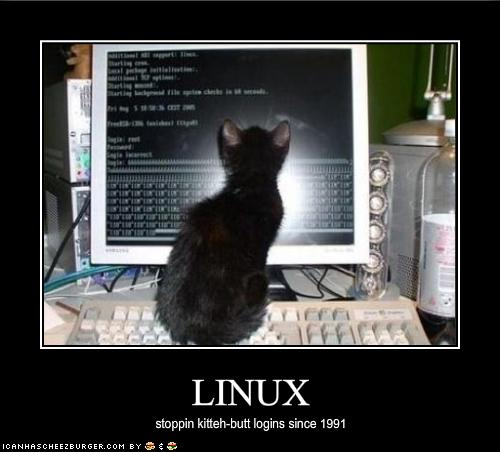
\includegraphics[scale=0.35]{resources/kitteh.jpg}
\end{figure}
\begin{itemize}
	\item Sicherheit
	\item Modifizierbarkeit
	\item kostenlos
\end{itemize}
%\footnote{http://danlynch.org/wp-content/uploads/2009/04/funny-pictures-your-kitten-uses-linux.jpg}
\end{frame}

\end{document}